\documentclass[11pt,a4paper]{article}
\usepackage[utf8]{inputenc}
\usepackage[T1]{fontenc}
\IfFileExists{lmodern.sty}{\usepackage{lmodern}}{}
\IfFileExists{spanish.ldf}{\usepackage[spanish,es-noshorthands]{babel}}{}
\usepackage{amsmath,amssymb,amsthm,mathtools}
\usepackage{enumitem}
\usepackage[margin=2.5cm]{geometry}
\usepackage{tikz}
\usepackage{booktabs}
\usepackage[colorlinks=true,linkcolor=blue!50!black,urlcolor=blue!50!black]{hyperref}
\setlength{\parskip}{3pt}
\linespread{1.04}

\newcommand{\Spec}{\operatorname{Spec}}
\newcommand{\Spm}{\operatorname{Spm}}
\newcommand{\Proj}{\operatorname{Proj}}
\newcommand{\Frac}{\operatorname{Frac}}
\newcommand{\Anu}{\operatorname{Anu}}
\newcommand{\Bl}{\operatorname{Bl}}
\newcommand{\gr}{\operatorname{gr}}
\newcommand{\nil}{\operatorname{nil}}
\newcommand{\hgt}{\operatorname{ht}}
\newcommand{\A}{\mathbb{A}}
\newcommand{\PP}{\mathbb{P}}
\newcommand{\ZZ}{\mathbb{Z}}
\newcommand{\QQ}{\mathbb{Q}}
\newcommand{\RR}{\mathbb{R}}
\newcommand{\CC}{\mathbb{C}}
\newcommand{\FF}{\mathbb{F}}
\newcommand{\pp}{\mathfrak{p}}
\newcommand{\qq}{\mathfrak{q}}
\newcommand{\mm}{\mathfrak{m}}
\newcommand{\aaa}{\mathfrak{a}}
\newcommand{\bbb}{\mathfrak{b}}

\theoremstyle{plain}
\newtheorem{teorema}{Teorema}[section]
\newtheorem{proposicion}[teorema]{Proposición}
\newtheorem{lema}[teorema]{Lema}
\newtheorem{corolario}[teorema]{Corolario}
\theoremstyle{definition}
\newtheorem{definicion}[teorema]{Definición}
\newtheorem{ejemplo}[teorema]{Ejemplo}
\theoremstyle{remark}
\newtheorem*{obs}{Observación}
\newtheorem*{docente}{Para el docente}

\newcounter{ej}
\newenvironment{ejercicio}[1][]{\refstepcounter{ej}\par\medskip\noindent\textbf{Ejercicio \theej}\ifx&#1&\else\ (#1)\fi.\ }{\par}
\newcommand{\libro}[1]{\textsc{[Palacios, #1]}}
\newcommand{\pregunta}[1]{\par\smallskip\noindent\fbox{\parbox{0.94\linewidth}{\textbf{Pregunta para la clase.} #1}}\par\smallskip}

\title{\textbf{Clase: El espectro de un anillo}\\[4pt]
\large Capítulo 5 de J.~Palacios, \emph{Geometría algebraica: esquemas y haces coherentes}\\
Curso de posgrado en geometría algebraica --- sesión de 3 horas}
\author{}
\date{Octubre de 2026}

\begin{document}
\maketitle

\section*{Ficha de la clase}

\paragraph{Público.} Estudiantes que han llevado un curso de álgebra de pregrado: grupos, anillos, ideales, anillos cociente, dominios, cuerpos de fracciones, DIP y DFU, anillos de polinomios. \emph{No} se supone álgebra conmutativa ni geometría algebraica: lo necesario (ideales primos, radical, localización, graduación) se repasa donde aparece.

\paragraph{Objetivos.} Al terminar, el estudiante podrá:
\begin{enumerate}[itemsep=1pt]
\item calcular el espectro de anillos concretos ($\ZZ$, $k[x]$, $k[x,y]$, cocientes y localizaciones) e identificar puntos cerrados, puntos genéricos, cierres y componentes irreducibles;
\item demostrar que $V(\aaa)$ define una topología y manejar el diccionario \emph{ideales radicales $\leftrightarrow$ cerrados};
\item explicar por qué un homomorfismo de anillos induce una aplicación continua en sentido contrario, y reconocer cuándo da una inmersión cerrada o un abierto;
\item describir $\Proj$ de un anillo graduado, calcular sus puntos y sus cartas $D_+(f)$.
\end{enumerate}

\paragraph{Cronograma.}
\begin{center}
\begin{tabular}{@{}lll@{}}
\toprule
Bloque & Contenido & Tiempo \\
\midrule
0 & Motivación: de variedades a anillos & 10 min \\
1 & $\Spec A$: conjunto, topología, puntos genéricos & 45 min \\
2 & Dimensión y abiertos básicos $D(a)$ & 20 min \\
\multicolumn{3}{c}{\emph{pausa (10 min)}} \\
3 & Homomorfismos de anillos y aplicaciones continuas & 40 min \\
4 & El espectro proyectivo $\Proj S$ & 35 min \\
5 & Ejercicios en clase y cierre & 20 min \\
\bottomrule
\end{tabular}
\end{center}

\paragraph{Convenciones.} Todos los anillos son conmutativos con unidad. $k$ es un cuerpo; cuando se diga \emph{algebraicamente cerrado} se indicará. Se indica con \libro{Ej.~5.1.3} el ejemplo del libro correspondiente. Las notas \emph{Para el docente} sugieren cómo conducir la clase; el estudiante puede ignorarlas.

\section{Bloque 0. Motivación (10 min)}

\paragraph{Una observación sobre la recta.} Sea $k$ algebraicamente cerrado. Los puntos de $\A^1=k$ se corresponden con los ideales maximales de $k[x]$: $a\leftrightarrow(x-a)$. Un polinomio $f$ ``vale cero en $a$'' si y sólo si $f\in(x-a)$. Así la geometría de $k$ está codificada en el anillo $k[x]$.

\paragraph{El problema.} Queremos hacer lo mismo para \emph{cualquier} anillo, incluso $\ZZ$ o $k[x]/(x^2)$. ¿Qué son los ``puntos'' de $\ZZ$? ¿Y de $k[x]/(x^2)$? Probamos con los ideales maximales, y aparece un defecto:

\begin{ejemplo}[{Los maximales no son funtoriales}]\label{ej:no-max}
La inclusión $\varphi:\ZZ\hookrightarrow\QQ$ es un homomorfismo. El ideal $(0)$ es maximal en $\QQ$ (es un cuerpo), pero $\varphi^{-1}(0)=(0)$ no es maximal en $\ZZ$. De manera análoga, $k[x]\hookrightarrow k(x)$.
\end{ejemplo}

En cambio, la imagen inversa de un ideal \emph{primo} sigue siendo primo.

\begin{lema}\label{lema:contraccion}
Sea $\varphi:A\to B$ un homomorfismo y $\qq\subset B$ primo. Entonces $\varphi^{-1}(\qq)$ es primo.
\end{lema}
\begin{proof}
$1\notin\varphi^{-1}(\qq)$ porque $\varphi(1)=1\notin\qq$. Si $ab\in\varphi^{-1}(\qq)$, entonces $\varphi(a)\varphi(b)\in\qq$, luego $\varphi(a)\in\qq$ o $\varphi(b)\in\qq$.
\end{proof}

\noindent\textbf{Moraleja:} el conjunto de \emph{todos} los primos, y no sólo de los maximales, es el que hace de $A\mapsto\{\text{puntos}\}$ un funtor (en sentido contrario). Ese conjunto es el espectro.

\begin{docente}
Dibujar en el pizarrón $\ZZ\subset\QQ$ y preguntar: ``¿a qué punto de $\Spec\ZZ$ debe ir el único punto de $\Spec\QQ$?'' Respuesta esperada tras unos minutos: a $(0)$, y por eso $(0)$ debe ser un punto aunque no sea maximal. Esto motiva los \emph{puntos genéricos}.
\end{docente}

\section{Bloque 1. El espectro afín (45 min)}

\subsection{Repaso: primos, maximales y radical}

\begin{definicion}
Sea $A$ un anillo. Un ideal $\pp\ne A$ es \emph{primo} si $ab\in\pp\Rightarrow a\in\pp$ o $b\in\pp$ (equivale a que $A/\pp$ sea dominio). Un ideal $\mm\ne A$ es \emph{maximal} si no hay ideales propios que lo contengan estrictamente (equivale a que $A/\mm$ sea cuerpo). El \emph{radical} de un ideal $\aaa$ es $\sqrt\aaa=\{a:a^n\in\aaa\text{ para algún }n\ge1\}$; el \emph{nilradical} de $A$ es $\nil(A)=\sqrt{(0)}$.
\end{definicion}

Todo maximal es primo (un cuerpo es dominio). El siguiente resultado es la herramienta técnica del capítulo.

\begin{teorema}[{El radical es la intersección de los primos}]\label{teo:radical}
Para todo ideal propio $\aaa$ de $A$, $\sqrt\aaa=\bigcap_{\pp\supseteq\aaa}\pp$.
\end{teorema}
\begin{proof}
($\subseteq$) Si $a^n\in\aaa\subseteq\pp$, entonces $a\in\pp$ por primalidad.

($\supseteq$) Sea $f\notin\sqrt\aaa$; hay que hallar un primo $\pp\supseteq\aaa$ con $f\notin\pp$. Sea $S=\{1,f,f^2,\dots\}$; por hipótesis $S\cap\aaa=\varnothing$. Por el lema de Zorn existe un ideal $\pp$ maximal entre los que contienen a $\aaa$ y no cortan a $S$. Veamos que es primo: si $x,y\notin\pp$, entonces $\pp+(x)$ y $\pp+(y)$ cortan a $S$: $f^m=p_1+rx$, $f^n=p_2+ty$, y multiplicando $f^{m+n}\in\pp+(xy)$. Luego $\pp+(xy)$ corta a $S$ y por tanto $xy\notin\pp$. Así $\pp$ es primo, contiene a $\aaa$ y no contiene a $f$.
\end{proof}

\begin{docente}
No hay que escribir toda la prueba de Zorn en clase; basta la idea: ``si $f$ no es nilpotente módulo $\aaa$, existe un primo que contiene a $\aaa$ y evita a $f$''. Pedir que los estudiantes verifiquen el caso $A=\ZZ$, $\aaa=(12)$: $\sqrt{(12)}=(6)=(2)\cap(3)$.
\end{docente}

\subsection{Definición del espectro}

\begin{definicion}[{\libro{Def.~5.1.1}}]
El \emph{espectro} de $A$ es el conjunto $\Spec A$ de ideales primos de $A$. Para $S\subseteq A$,
\[
V(S)=\{\pp\in\Spec A:S\subseteq\pp\}.
\]
Si $\aaa=\langle S\rangle$, entonces $V(S)=V(\aaa)=V(\sqrt\aaa)$.
\end{definicion}

\paragraph{Lectura geométrica.} Un elemento $a\in A$ es una ``función'' sobre $\Spec A$, y $a$ ``se anula en $\pp$'' si $a\in\pp$. Entonces $V(S)$ es el \emph{conjunto de ceros comunes} de $S$.

\begin{ejemplo}[{Cuatro espectros fundamentales, \libro{Ej.~5.1.1--5.1.4}}]\label{ej:cuatro}
\begin{enumerate}[label=(\alph*),itemsep=2pt]
\item \emph{Un cuerpo $k$.} Los ideales de $k$ son $(0)$ y $k$ (si $a\ne0$ está en $I$, entonces $1=a^{-1}a\in I$). El único primo es $(0)$: $\Spec k$ es un punto.
\item \emph{Un anillo de valuación discreta $A$} (por ejemplo $\ZZ_{(p)}$ o $k[x]_{(x)}$). Tiene exactamente dos primos: $\eta=(0)$ y $s=\mm$. Son el \emph{punto genérico} y el \emph{punto especial}.
\item \emph{$\ZZ$.} Primos: $(0)$ y $(p)$, $p$ primo. Dibujo:
\begin{center}
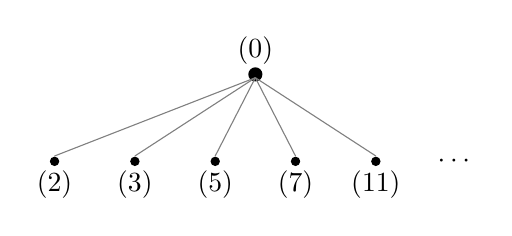
\begin{tikzpicture}[scale=0.85]
 \fill (0,1.3) circle (3pt) node[above]{$(0)$};
 \foreach \x/\l in {-3/2,-1.8/3,-0.6/5,0.6/7,1.8/11}{
   \fill (\x,0) circle (2pt) node[below]{$(\l)$};
   \draw[gray,thin] (0,1.25)--(\x,0.08);
 }
 \node at (3.0,0) {$\cdots$};
\end{tikzpicture}
\end{center}
\item \emph{$K[x]$.} Primos: $(0)$ y $(f)$ con $f$ irreducible. Si $K=k$ es algebraicamente cerrado, $f=x-a$ y los puntos cerrados son $a\in k$. En $\RR[x]$, el primo $(x^2+1)$ es un punto cerrado que ``representa a la vez a $i$ y $-i$''.
\end{enumerate}
\end{ejemplo}

\pregunta{¿Cuántos puntos tiene $\Spec k[x]/(x^2)$? ¿Y $\Spec k[x]/(x^2-x)$? (Pista: los primos de un cociente $A/\aaa$ son los primos de $A$ que contienen a $\aaa$.)}

\emph{Respuesta.} $k[x]/(x^2)$: sólo $(x)$, un punto. $k[x]/(x^2-x)=k[x]/(x(x-1))$: dos puntos, $(x)$ y $(x-1)$. Como \emph{conjuntos} el primero es indistinguible de $\Spec k$; se distingue por el anillo de funciones $k[\varepsilon]$, que no es reducido: esa información es la que recoge el haz estructural (Cap.~7).

\subsection{La topología de Zariski}

\begin{proposicion}[{\libro{Prop.~5.1.5}}]\label{prop:cerrados}
En $X=\Spec A$:
\begin{enumerate}[label=(\alph*),itemsep=1pt]
\item $V(0)=X$ y $V(1)=\varnothing$;
\item $V(\aaa_1\aaa_2)=V(\aaa_1\cap\aaa_2)=V(\aaa_1)\cup V(\aaa_2)$;
\item $\bigcap_iV(\aaa_i)=V\!\big(\sum_i\aaa_i\big)$.
\end{enumerate}
\end{proposicion}
\begin{proof}
(a) Todo primo contiene a $0$ y ninguno contiene a $1$. (c) $\pp$ contiene a todos los $\aaa_i$ si y sólo si contiene a su suma. (b) Como $\aaa_1\aaa_2\subseteq\aaa_1\cap\aaa_2$, $V(\aaa_1\cap\aaa_2)\subseteq V(\aaa_1\aaa_2)$; y $V(\aaa_1)\cup V(\aaa_2)\subseteq V(\aaa_1\cap\aaa_2)$ es claro. Falta $V(\aaa_1\aaa_2)\subseteq V(\aaa_1)\cup V(\aaa_2)$: si $\pp\supseteq\aaa_1\aaa_2$ y $\aaa_1\not\subseteq\pp$, hay $a\in\aaa_1\setminus\pp$ y para cada $b\in\aaa_2$, $ab\in\pp\Rightarrow b\in\pp$; luego $\aaa_2\subseteq\pp$.
\end{proof}

\begin{definicion}
La \emph{topología de Zariski} (o espectral) sobre $\Spec A$ es aquella cuyos cerrados son los $V(\aaa)$.
\end{definicion}

\subsection{El diccionario entre cerrados e ideales}

Para $Y\subseteq X$ se define $I(Y)=\bigcap_{\pp\in Y}\pp$, un ideal radical.

\begin{proposicion}[{\libro{Lema~5.1.6}}]\label{prop:dicc}
\begin{enumerate}[label=(\alph*),itemsep=1pt]
\item $I(V(\aaa))=\sqrt\aaa$ para todo ideal $\aaa$.
\item $V(I(Y))=\overline Y$ (la clausura de Zariski de $Y$).
\item $V(\aaa)\subseteq V(\bbb)\iff\sqrt\bbb\subseteq\sqrt\aaa$. En particular $V(\aaa)=V(\bbb)\iff\sqrt\aaa=\sqrt\bbb$.
\end{enumerate}
\end{proposicion}
\begin{proof}
(a) Es el Teorema~\ref{teo:radical} (si $\aaa=A$ ambos lados son $A$). (b) $V(I(Y))$ es un cerrado que contiene a $Y$. Si $V(\aaa)\supseteq Y$, todo primo de $Y$ contiene a $\aaa$, así que $\aaa\subseteq I(Y)$ y $V(I(Y))\subseteq V(\aaa)$. Luego $V(I(Y))$ es el menor cerrado que contiene a $Y$. (c) Por (a): $V(\aaa)\subseteq V(\bbb)\Rightarrow I(V(\bbb))\subseteq I(V(\aaa))$, es decir $\sqrt\bbb\subseteq\sqrt\aaa$. La recíproca es inmediata.
\end{proof}

\paragraph{Consecuencia.} $\aaa\mapsto V(\aaa)$ es una biyección que invierte inclusiones entre \emph{ideales radicales} de $A$ y \emph{cerrados} de $\Spec A$. Esto es el Nullstellensatz \emph{sin hipótesis}: en un espectro cuentan todos los primos.

\begin{corolario}[{\libro{Cor.~5.1.8}: especialización}]\label{cor:espec}
Para $x,y\in\Spec A$ (con primos $\pp_x,\pp_y$):
\begin{enumerate}[label=(\alph*),itemsep=1pt]
\item $\overline{\{x\}}=V(\pp_x)$;
\item $\{x\}$ es cerrado $\iff\pp_x$ es maximal;
\item $y\in\overline{\{x\}}\iff\pp_x\subseteq\pp_y$ (se dice que $y$ es una \emph{especialización} de $x$);
\item $x$ es \emph{genérico} (su clausura es una componente irreducible) $\iff\pp_x$ es primo minimal.
\end{enumerate}
\end{corolario}
\begin{proof}
(a) Por la Proposición~\ref{prop:dicc}(b), $\overline{\{x\}}=V(I(\{x\}))=V(\pp_x)$. (c) es la definición de $V(\pp_x)$. (b) $\{x\}=V(\pp_x)$ equivale a que $\pp_x$ no esté contenido estrictamente en otro primo; como todo ideal propio está contenido en un maximal (que es primo), eso equivale a que $\pp_x$ sea maximal. (d) se sigue de (c) y de la Proposición~\ref{prop:irred} siguiente.
\end{proof}

\paragraph{Regla mnemotécnica.} \emph{Primo pequeño $=$ punto grande (genérico). Primo grande $=$ punto pequeño (cerrado).} En $\Spec\ZZ$: $(0)$ es el punto cuya clausura es todo.

\subsection{Irreducibilidad y puntos genéricos}

Un espacio topológico $Z\neq\varnothing$ es \emph{irreducible} si no es unión de dos cerrados propios.

\begin{proposicion}[{\libro{Cor.~5.1.10}}]\label{prop:irred}
\begin{enumerate}[label=(\alph*),itemsep=1pt]
\item $V(\aaa)$ es irreducible $\iff\sqrt\aaa$ es primo. En particular $\Spec A$ es irreducible $\iff\nil(A)$ es primo.
\item Todo cerrado irreducible de $\Spec A$ tiene un \emph{único} punto genérico: es $V(\pp)=\overline{\{\pp\}}$.
\item Las componentes irreducibles de $\Spec A$ son las clausuras $V(\pp)$ de los primos minimales.
\end{enumerate}
\end{proposicion}
\begin{proof}
(a) ($\Leftarrow$) Sea $\pp=\sqrt\aaa$ primo y $V(\aaa)=V(\bbb_1)\cup V(\bbb_2)$. Entonces $V(\aaa)=V(\bbb_1\bbb_2)$, luego $\bbb_1\bbb_2\subseteq\sqrt\aaa=\pp$ y, por primalidad, $\bbb_1\subseteq\pp$ o $\bbb_2\subseteq\pp$, es decir $V(\aaa)=V(\pp)\subseteq V(\bbb_i)$. ($\Rightarrow$) Si $V(\aaa)$ es irreducible y $xy\in\sqrt\aaa$, entonces $V(\aaa)\subseteq V(xy)=V(x)\cup V(y)$, luego $V(\aaa)=(V(\aaa)\cap V(x))\cup(V(\aaa)\cap V(y))$ y por irreducibilidad $V(\aaa)\subseteq V(x)$ o $\subseteq V(y)$, es decir $x\in\sqrt\aaa$ o $y\in\sqrt\aaa$. Además $\sqrt\aaa\ne A$.

(b) Si $Z=V(\aaa)$ es irreducible, $\sqrt\aaa=\pp$ primo y $Z=V(\pp)=\overline{\{\pp\}}$. Unicidad: si $\overline{\{\pp\}}=\overline{\{\pp'\}}$, entonces $V(\pp)=V(\pp')$, luego $\pp=\pp'$ por la Proposición~\ref{prop:dicc}(c).

(c) Los cerrados irreducibles maximales corresponden, por (a) y la biyección, a los primos minimales.
\end{proof}

\begin{ejemplo}[{$\Spec k[x,y]/(xy)$, el nodo}]\label{ej:nodo5}
Los primos de $k[x,y]$ que contienen a $(xy)$ contienen a $(x)$ o a $(y)$. Primos minimales: $(x)$ y $(y)$ (puntos genéricos de los dos ejes). Hay otros primos $(x,y-b)$ ($b\ne0$), $(x-a,y)$ ($a\ne0$) y $(x,y)$ (el origen, que pertenece a la clausura de ambos genéricos). Hay \emph{dos} componentes irreducibles, $V(x)$ y $V(y)$: $\Spec A$ es conexo pero no irreducible.
\begin{center}
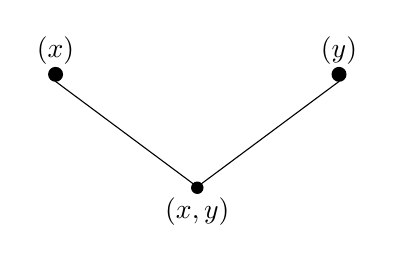
\begin{tikzpicture}[scale=0.9]
 \fill (0,0) circle (2.5pt) node[below]{$(x,y)$};
 \fill (-2,1.6) circle (3pt) node[above]{$(x)$};
 \fill (2,1.6) circle (3pt) node[above]{$(y)$};
 \draw (-2,1.5)--(-0.05,0.05); \draw (2,1.5)--(0.05,0.05);
\end{tikzpicture}
\end{center}
\end{ejemplo}

\begin{ejemplo}[{$\Spec k[x,y]$, $k$ algebraicamente cerrado}]\label{ej:plano5}
Hay tres tipos de primos: $(0)$ (genérico del plano, clausura de dimensión $2$); $(f)$ con $f$ irreducible (genérico de una curva, clausura de dimensión $1$); $(x-a,y-b)$ (puntos cerrados). La cadena $(0)\subset(y-x^2)\subset(x,y)$ lee ``el origen está en la parábola, que está en el plano''.
\end{ejemplo}

\begin{ejemplo}[{La curva de Fermat sobre $\ZZ$, \libro{Ej.~5.1.11}}]
$x^n+y^n-z^n$ es irreducible en $\ZZ[x,y,z]$, luego $V(x^n+y^n-z^n)\subset\Spec\ZZ[x,y,z]$ es irreducible por la Proposición~\ref{prop:irred}(a). Es irreducible ``sobre todos los primos a la vez'': contiene curvas sobre cada $\FF_p$ y sobre $\QQ$.
\end{ejemplo}

\begin{docente}
Conviene detener la clase aquí 2 minutos y hacer un cuadro de equivalencias en el pizarrón: \emph{cerrado irreducible $\leftrightarrow$ primo; punto cerrado $\leftrightarrow$ maximal; componente irreducible $\leftrightarrow$ primo minimal; punto en la clausura de otro $\leftrightarrow$ inclusión de primos}. Es el vocabulario del curso.
\end{docente}

\section{Bloque 2. Dimensión y abiertos básicos (20 min)}

\subsection{Dimensión}

La \emph{dimensión} de un espacio topológico es el supremo de las longitudes $n$ de cadenas $Z_0\subsetneq Z_1\subsetneq\cdots\subsetneq Z_n$ de cerrados irreducibles. Por la Proposición~\ref{prop:irred}, $Z_i=V(\pp_i)$ y la cadena equivale a $\pp_0\supsetneq\pp_1\supsetneq\cdots\supsetneq\pp_n$.

\begin{proposicion}[{\libro{Sec.~5.2}}]
$\dim\Spec A=\dim A$ (dimensión de Krull).
\end{proposicion}

\begin{ejemplo}
$\dim\Spec k=0$; $\dim\Spec\ZZ=1$; un DVR tiene dimensión $1$ (\libro{Ej.~5.2.1}); $\dim\Spec k[x,y]=2$ por la cadena $(0)\subset(x)\subset(x,y)$; $\dim\Spec\ZZ[x]=2$ por $(0)\subset(x)\subset(2,x)$. ¿Y $\Spec k[x,y]/(xy)$? Tiene dimensión $1$.
\end{ejemplo}

\subsection{Abiertos básicos}

\begin{definicion}
Para $a\in A$, $D(a)=X\setminus V(a)=\{\pp:a\notin\pp\}$ (los puntos donde $a$ ``no se anula'').
\end{definicion}

\begin{proposicion}[{\libro{Prop.~5.2.2}}]\label{prop:Da}
\begin{enumerate}[label=(\alph*),itemsep=1pt]
\item Los $D(a)$ forman una base de la topología.
\item $D(a)\cap D(b)=D(ab)$.
\item $D(a)=\varnothing\iff a$ es nilpotente; $D(a)=X\iff a$ es unidad.
\item $D(a)$ es \emph{casi compacto}: todo cubrimiento por abiertos admite un subcubrimiento finito.
\end{enumerate}
\end{proposicion}
\begin{proof}
(a) Todo abierto es $X\setminus V(\aaa)=\bigcup_{a\in\aaa}D(a)$, pues $V(\aaa)=\bigcap_{a\in\aaa}V(a)$.
(b) $\pp\not\ni ab\iff\pp\not\ni a$ y $\pp\not\ni b$ (primalidad).
(c) $D(a)=\varnothing\iff a\in\bigcap\pp=\nil(A)$ (Teorema~\ref{teo:radical}); $D(a)=X\iff a$ no está en ningún maximal $\iff a$ es unidad.
(d) Basta cubrimientos por básicos: $D(a)\subseteq\bigcup_{i\in I}D(a_i)$. Sea $\aaa=(a_i)_{i\in I}$. Entonces $V(\aaa)=\bigcap V(a_i)\subseteq V(a)$, así que $a\in\sqrt\aaa$ (Prop.~\ref{prop:dicc}(c)): $a^n=\sum_{j=1}^r\alpha_ja_{i_j}$ con \emph{finitos} términos. Luego $V(a_{i_1},\dots,a_{i_r})\subseteq V(a^n)=V(a)$ y $D(a)\subseteq D(a_{i_1})\cup\cdots\cup D(a_{i_r})$.
\end{proof}

\begin{ejemplo}[{Un abierto no casi compacto}]
Sea $A=k[x_1,x_2,\dots]$ con infinitas variables y $\mm=(x_1,x_2,\dots)$. El abierto $U=X\setminus V(\mm)=\bigcup_iD(x_i)$ no es casi compacto: $\pp=(x_1,\dots,x_r)\in U$ no está en $D(x_1)\cup\cdots\cup D(x_r)$. En anillos noetherianos esto no ocurre (todo abierto es casi compacto).
\end{ejemplo}

\paragraph{Nota.} ``Casi compacto'' es compacto sin la hipótesis de Hausdorff. De hecho $\Spec A$ casi nunca es Hausdorff: en $\Spec\ZZ$ el punto $(0)$ está en la clausura de todos los demás.

\begin{docente}
Pausa de 10 minutos después de este bloque.
\end{docente}

\section{Bloque 3. Homomorfismos de anillos y aplicaciones continuas (40 min)}

\subsection{La aplicación inducida}

Sea $\varphi:A\to B$ un homomorfismo, $X=\Spec A$, $Y=\Spec B$. Por el Lema~\ref{lema:contraccion} está bien definida
\[
\varphi^*:Y\to X,\qquad\qq\mapsto\varphi^{-1}(\qq).
\]

\begin{proposicion}[{\libro{Prop.~5.3.1}}]\label{prop:phi}
\begin{enumerate}[label=(\alph*),itemsep=2pt]
\item $(\varphi^*)^{-1}(D(f))=D(\varphi(f))$ para $f\in A$.
\item $(\varphi^*)^{-1}(V(\aaa))=V(\varphi(\aaa)B)$ para todo ideal $\aaa\subseteq A$. En particular $\varphi^*$ es continua.
\item (\emph{Funtorialidad}) $(\psi\circ\varphi)^*=\varphi^*\circ\psi^*$.
\item Si $\varphi$ es \emph{sobreyectivo}, $\varphi^*$ es un homeomorfismo de $Y$ sobre el cerrado $V(\ker\varphi)$.
\item La clausura de la imagen es $\overline{\varphi^*(Y)}=V(\ker\varphi)$. En particular $\varphi^*(Y)$ es denso $\iff\ker\varphi\subseteq\nil(A)$.
\end{enumerate}
\end{proposicion}
\begin{proof}
(a) $\qq\in(\varphi^*)^{-1}(D(f))\iff f\notin\varphi^{-1}(\qq)\iff\varphi(f)\notin\qq$.

(b) $\qq\in(\varphi^*)^{-1}(V(\aaa))\iff\aaa\subseteq\varphi^{-1}(\qq)\iff\varphi(\aaa)\subseteq\qq\iff\varphi(\aaa)B\subseteq\qq$. Como los $V(\aaa)$ son los cerrados, $\varphi^*$ es continua.

(c) $(\varphi^*\circ\psi^*)(\mathfrak r)=\varphi^{-1}(\psi^{-1}(\mathfrak r))=(\psi\varphi)^{-1}(\mathfrak r)$.

(d) Si $\varphi$ es sobreyectivo, $B\cong A/\ker\varphi$ y, por el teorema de correspondencia, los primos de $B$ se corresponden con los primos de $A$ que contienen a $\ker\varphi$, y esta correspondencia es $\qq\mapsto\varphi^{-1}(\qq)$. Es biyectiva sobre $V(\ker\varphi)$, continua por (b), y su inversa es $\pp\mapsto\varphi(\pp)$, que lleva el cerrado $V(\bbb)$ de $Y$ al cerrado $V(\varphi^{-1}(\bbb))\subseteq X$ (de nuevo por correspondencia): es cerrada.

(e) $I(\varphi^*(Y))=\bigcap_\qq\varphi^{-1}(\qq)=\varphi^{-1}\big(\bigcap_\qq\qq\big)=\varphi^{-1}(\nil B)=\sqrt{\ker\varphi}$, pues $\varphi(a)$ es nilpotente $\iff a^n\in\ker\varphi$. Por la Proposición~\ref{prop:dicc}(b), $\overline{\varphi^*(Y)}=V(\sqrt{\ker\varphi})=V(\ker\varphi)$.
\end{proof}

\begin{obs}
Una versión más fuerte de (e) (que $\varphi^*(V(\bbb))=V(\varphi^{-1}(\bbb))$ para todo $\bbb$) es \emph{falsa} en general: sólo vale para la \emph{clausura} de $\varphi^*(V(\bbb))$. Contraejemplo: $\varphi:k[x]\to k[x]_x$ y $\bbb=0$: $\varphi^*(Y)=D(x)$ no es cerrado y $V(\varphi^{-1}(0))=V(0)=\A^1$. La imagen se vuelve cerrada si $\varphi$ es entero (teorema de ``going up''), como en la normalización de curvas.
\end{obs}

\subsection{Ejemplos}

\begin{ejemplo}[{Cociente $\Rightarrow$ cerrado: $k[x]\to k[x]/(x^2)$}]\label{ej:cociente}
Por (d), $\Spec k[x]/(x^2)\to\Spec k[x]$ es un homeomorfismo sobre $V(x^2)=\{(x)\}$, el origen. Pero $V(x^2)=V(x)$ como \emph{conjuntos}. El homomorfismo $k[x]\to k[x]/(x)$ da el mismo conjunto: la inmersión cerrada es \emph{distinta} (``punto doble'' versus ``punto'').
\end{ejemplo}

\begin{ejemplo}[{Fibras y preimágenes: $t\mapsto xy$}]\label{ej:fibra}
$\varphi:k[t]\to k[x,y]$, $t\mapsto xy$. Por (a) y (b): $(\varphi^*)^{-1}(V(t))=V(xy)$, la cruz de los dos ejes, y $(\varphi^*)^{-1}(D(t))=D(xy)$. Como $\ker\varphi=0$, la imagen es densa (e). Las fibras $\{xy=a\}$ son hipérbolas para $a\ne0$ y la cruz para $a=0$.
\end{ejemplo}

\begin{ejemplo}[{Normalización de la cúspide: homeomorfismo que no es isomorfismo}]\label{ej:cuspide}
$\iota:k[t^2,t^3]\hookrightarrow k[t]$ induce $\iota^*:\A^1\to C=\Spec k[t^2,t^3]$, $a\mapsto(a^2,a^3)$. Los maximales de $k[t^2,t^3]$ son $\mm_a=(t^2-a^2,t^3-a^3)$ y $\iota^{-1}((t-a))=\mm_a$; además $\iota^{-1}(0)=0$. Así $\iota^*$ es biyectiva; como $k[t]$ es entero sobre $k[t^2,t^3]$, es cerrada, luego un homeomorfismo. Pero $\iota$ no es sobreyectivo ($t\notin k[t^2,t^3]$): no es isomorfismo. Se distinguen por el espacio tangente: $\dim\mm_0/\mm_0^2=2$ para la cúspide y $1$ para $k[t]$.
\end{ejemplo}

\begin{ejemplo}[{Biyección continua que no es homeomorfismo, \libro{Prop.~5.3.1(g)}}]\label{ej:zp}
Sea $A=\ZZ_{(p)}$ (DVR con primos $(0)$ y $(p)$), $K=\QQ$, $B=\FF_p\times\QQ$ y $\varphi(x)=([x],x)$.
\begin{itemize}[itemsep=1pt]
\item $B$ es producto de dos cuerpos: sus primos son $\qq_1=\{(a,0)\}$ y $\qq_2=\{(0,b)\}$, ambos maximales. $\Spec B$ es discreto.
\item $\varphi^{-1}(\qq_1)=(0)$ y $\varphi^{-1}(\qq_2)=(p)$: $\varphi^*$ es biyectiva y continua.
\item $\Spec\ZZ_{(p)}=\{(0),(p)\}$ con $\{(0)\}$ \emph{abierto no cerrado}. Pero $\{\qq_1\}$ es cerrado y su imagen $\{(0)\}$ no lo es. Luego $\varphi^*$ no es cerrada y no es homeomorfismo.
\end{itemize}
Moraleja: la topología de $\Spec A$ ``pega'' la fibra genérica $\Spec\QQ$ y la fibra especial $\Spec\FF_p$ de una manera que no se ve en el conjunto de puntos.
\end{ejemplo}

\subsection{Localización: los abiertos básicos son espectros}

\begin{proposicion}[{\libro{Prop.~5.3.2}}]\label{prop:loc}
Sea $S\subseteq A$ multiplicativo y $\varphi:A\to S^{-1}A$. Entonces $\varphi^*$ es un homeomorfismo de $\Spec S^{-1}A$ sobre $\{\pp\in\Spec A:\pp\cap S=\varnothing\}$. En particular, si $S=\{1,f,f^2,\dots\}$, $\Spec A_f\cong D(f)$.
\end{proposicion}
\begin{proof}[Idea de la demostración]
Los primos de $S^{-1}A$ son exactamente los $\pp S^{-1}A$ con $\pp$ primo de $A$ y $\pp\cap S=\varnothing$, y $\pp\mapsto\pp S^{-1}A$ y $\qq\mapsto\varphi^{-1}(\qq)$ son inversas (porque $\pp=\pp^{ec}$ si $\pp\cap S=\varnothing$). La continuidad de la inversa sigue de $V(\bbb)\cap\operatorname{Im}=V(\bbb^c)\cap\operatorname{Im}$ para $\bbb\subseteq S^{-1}A$. Finalmente $\pp\cap\{f^n\}=\varnothing\iff f\notin\pp$, es decir $\pp\in D(f)$.
\end{proof}

\begin{ejemplo}[{Dos localizaciones de $k[x]$}]\label{ej:loc}
\begin{itemize}[itemsep=1pt]
\item $S=\{x^n\}$: $\Spec k[x]_x=\Spec k[x,x^{-1}]\cong D(x)=\A^1\setminus\{0\}$, abierto.
\item $S=k[x]\setminus(x)$: $\Spec k[x]_{(x)}\cong\{\pp:\pp\subseteq(x)\}=\{(0),(x)\}$, con la topología de Sierpinski. Es el ``germen en $0$'': \emph{no} es abierto de $\A^1$ (todo abierto no vacío contiene infinitos puntos). Representa a todos los abiertos alrededor de $0$ a la vez.
\end{itemize}
\end{ejemplo}

\begin{ejemplo}[{Anticipo del blow-up: $\pi$ es un isomorfismo fuera del centro}]\label{ej:antic}
Sea $A=k[x,y]$ y $A[y/x]=k[x,s]$ la carta del blow-up del origen. El homomorfismo $A\to A[y/x]$ es $y\mapsto xs$. Si se invierte $x$, ambos anillos coinciden: $A_x=A[y/x]_x$. Por la Proposición~\ref{prop:loc}, $\pi$ restringido a $\{x\ne0\}$ es un isomorfismo sobre $D(x)=\A^2\setminus\{x=0\}$. Por simetría, $\pi$ es isomorfismo sobre $\A^2\setminus\{0\}$.
\end{ejemplo}

\section{Bloque 4. El espectro proyectivo (35 min)}

\subsection{Motivación y definición}

En $\PP^n$, los polinomios no son funciones, pero los \emph{polinomios homogéneos} tienen un conjunto de ceros bien definido. Esto sugiere reemplazar $k[x_0,\dots,x_n]$ por un anillo graduado.

\begin{definicion}
Un \emph{anillo graduado} es un anillo $S=\bigoplus_{d\ge0}S_d$ con $S_dS_e\subseteq S_{d+e}$. Los elementos de $S_d$ son \emph{homogéneos de grado $d$}. El \emph{ideal irrelevante} es $S_+=\bigoplus_{d>0}S_d$. Un ideal es \emph{homogéneo} si está generado por elementos homogéneos.
\end{definicion}

\begin{definicion}[{\libro{Def.~5.4.1}}]
$\Proj S$ es el conjunto de ideales primos \emph{homogéneos} $\pp\subset S$ con $S_+\not\subseteq\pp$. Para $\aaa$ homogéneo, $V_+(\aaa)=\{\pp\in\Proj S:\aaa\subseteq\pp\}$; los $V_+(\aaa)$ son los cerrados de la topología de Zariski (el análogo de la Proposición~\ref{prop:cerrados}). Para $f\in S_+$ homogéneo, $D_+(f)=\{\pp:f\notin\pp\}$ es abierto, y estos forman una base.
\end{definicion}

\paragraph{Por qué excluir los primos que contienen a $S_+$.} El único primo homogéneo maximal $S_+=(x_0,\dots,x_n)$ en $k[x_0,\dots,x_n]$ corresponde al \emph{origen} del cono $\A^{n+1}$, que no es un punto de $\PP^n$. Y más en general, todo primo que contiene a $S_+$ es ``irrelevante'' porque todos los polinomios homogéneos de grado positivo se anulan en él.

\subsection{Propiedades básicas}

\begin{proposicion}[{\libro{Prop.~5.4.1}}]\label{prop:5.4.1}
Un primo homogéneo $\pp\in\Proj S$ está determinado por $\pp\cap S_+$.
\end{proposicion}
\begin{proof}
Como $S_+\not\subseteq\pp$, hay $f\in S_+$ homogéneo, $f\notin\pp$, de grado $d>0$. Para $a\in S_0$: $a\in\pp\iff af\in\pp$ (porque $\pp$ es primo y $f\notin\pp$), y $af\in S_d\subseteq S_+$. Entonces $\pp\cap S_0$ se recupera de $\pp\cap S_+$, y $\pp$ es homogéneo, de modo que queda determinado por sus partes homogéneas.
\end{proof}

\begin{lema}[{\libro{Lema~5.4.3}: las cartas}]\label{lema:cartas}
Si $S$ está generado por $S_1$ como $S_0$-álgebra, entonces $\Proj S=\bigcup_{f\in S_1}D_+(f)$.
\end{lema}
\begin{proof}
Sea $\pp\in\Proj S$. Existe $g\in S_+$ homogéneo, $g\notin\pp$, de grado $d>0$. Como $S$ es generado por $S_1$, $g$ es una combinación $S_0$-lineal de monomios $f_{i_1}\cdots f_{i_d}$ con $f_{i_j}\in S_1$. Si todos los $f_i$ estuvieran en $\pp$, también lo estaría $g$; luego algún $f\in S_1$ cumple $f\notin\pp$, es decir $\pp\in D_+(f)$.
\end{proof}

\begin{lema}[{\libro{Lema~5.4.4}}]
$\Proj S=\varnothing\iff$ todo elemento de $S_+$ es nilpotente.
\end{lema}
\begin{proof}[Idea]
Si $S_+\subseteq\nil(S)$, todo primo contiene a $S_+$. Recíprocamente, si $f\in S_+$ homogéneo no es nilpotente, existe un primo homogéneo que no lo contiene (versión homogénea del Teorema~\ref{teo:radical}) y ese primo no contiene a $S_+$.
\end{proof}

\subsection{Ejemplos}

\begin{ejemplo}[{$\Proj k[x,y]=\PP^1$}]\label{ej:p1}
Un primo homogéneo de altura $1$ en el DFU $k[x,y]$ es generado por un irreducible homogéneo: una forma lineal $bx-ay$. El primo de altura $2$, $(x,y)=S_+$, se excluye. Así
\[
\Proj k[x,y]=\{(0)\}\cup\{(bx-ay):[a:b]\in\PP^1(k)\}:
\]
un punto genérico y un punto cerrado por cada punto de $\PP^1$ ($k$ algebraicamente cerrado). Cartas (Lema~\ref{lema:cartas}): $D_+(x)=\Spec k[y/x]$ y $D_+(y)=\Spec k[x/y]$, con $k[y/x,x/y]=k[s,s^{-1}]$ en la intersección.
\end{ejemplo}

\begin{ejemplo}[{Anillo con pesos: $\deg x=1$, $\deg y=2$}]\label{ej:pesos}
Los irreducibles homogéneos son $x$ y $y-\lambda x^2$ ($\lambda\in k$). $\Proj$ tiene los puntos $(0)$, $(x)$, $(y-\lambda x^2)$: otra recta proyectiva, con $\lambda\in\A^1$ y $(x)\leftrightarrow\lambda=\infty$. Aquí $S$ \emph{no} está generado por $S_1$: se necesitan $D_+(x)=\Spec k[y/x^2]$ y $D_+(y)=\Spec k[x^2/y]$ para cubrir. Este es el divisor excepcional del blow-up con pesos $(1,2)$.
\end{ejemplo}

\begin{ejemplo}[{$\Proj$ de una cónica}]
$S=k[x,y,z]/(xz-y^2)$ es el anillo de coordenadas del cono sobre una cónica. $\Spec S$ es una superficie (dimensión $2$) y $\Proj S$ la cónica (dimensión $1$): en general $\dim\Spec S=\dim\Proj S+1$ \libro{Ej.~5.5.8}. La cónica es un $\PP^1$ vía $[s:t]\mapsto[s^2:st:t^2]$ (Veronese).
\end{ejemplo}

\begin{ejemplo}[{Dos puntos: $\Proj k[x,y]/(xy)$}]
Los primos homogéneos de $k[x,y]$ que contienen a $(xy)$ y no a $(x,y)$ son $(x)$ y $(y)$. Luego $\Proj$ tiene dos puntos cerrados, $[0:1]$ y $[1:0]$. Compárese con $\Spec k[x,y]/(xy)$, que es el nodo con dimensión $1$.
\end{ejemplo}

\subsection{Módulos graduados y soporte}

Si $M$ es un $S$-módulo graduado y $\pp\in\Proj S$, se define $M_{(\pp)}$ como el conjunto de fracciones $m/g$ con $m\in M$ homogéneo, $g\in S\setminus\pp$ homogéneo y $\deg m=\deg g$. El \emph{soporte} es $\operatorname{supp}M=\{\pp:M_{(\pp)}\ne0\}$.

\begin{proposicion}[{\libro{Prop.~5.4.5}}]
Sea $S$ generado por $S_1$ sobre $S_0$ y $M$ un $S$-módulo graduado de tipo finito. Entonces:
\begin{enumerate}[label=(\alph*),itemsep=1pt]
\item $\operatorname{supp}M=V_+(\Anu M)$;
\item $M_d=0$ para todo $d\gg0$ $\iff M_{(\pp)}=0$ para todo $\pp\in\Proj S$.
\end{enumerate}
\end{proposicion}

\begin{ejemplo}[{Soportes}]\label{ej:soporte}
Sea $S=k[x,y,z]$.
\begin{center}
\begin{tabular}{@{}lll@{}}
\toprule
$M$ & $\Anu(M)$ & $\operatorname{supp}M$ \\
\midrule
$S/(f)$, $f$ homogéneo & $(f)$ & la curva $V_+(f)\subset\PP^2$ \\
$S/(x,y)$ & $(x,y)$ & el punto $[0:0:1]$ \\
$S/(x,y,z)=k$ & $S_+$ & $\varnothing$ \\
$S/(x,y,z)^3$ & $(x,y,z)^3$ & $\varnothing$ (se anula en grados $\ge3$) \\
\bottomrule
\end{tabular}
\end{center}
Los dos últimos módulos son ``invisibles'' en $\Proj$: es lo mismo que decir que $\Proj S$ no cambia si se ignoran los primeros grados.
\end{ejemplo}

\subsection{Un vistazo al blow-up}

Sea $A=k[x,y]$, $I=(x,y)$ y $R(I)=\bigoplus_{n\ge0}I^nt^n=A[xt,yt]$ (\emph{álgebra de Rees}). Es un anillo graduado con $R(I)_0=A$, generado por $R(I)_1=It$. Por el Lema~\ref{lema:cartas},
\[
\Proj R(I)=D_+(xt)\cup D_+(yt),\qquad D_+(xt)=\Spec R(I)_{(xt)}=\Spec A[y/x]=\Spec k[x,s].
\]
La inclusión $A=R(I)_0\to R(I)_{(xt)}$ induce el morfismo $\pi:\Proj R(I)\to\Spec A$. Es el \emph{blow-up del origen}. El Ejemplo~\ref{ej:antic} mostró que $\pi$ es un isomorfismo fuera del origen; sobre el origen la fibra es $\Proj\gr_I(A)=\Proj k[x,y]=\PP^1$ (Ejemplo~\ref{ej:p1}): el punto se reemplaza por la recta de las direcciones. Todo el desarrollo posterior del curso (blow-ups, transformada estricta, resolución de singularidades) se construye con las herramientas de este capítulo.

\section{Bloque 5. Ejercicios y cierre (20 min)}

\subsection*{Síntesis en una tabla}
\begin{center}
\begin{tabular}{@{}ll@{}}
\toprule
Álgebra & Geometría en $\Spec A$ \\
\midrule
ideal primo $\pp$ & punto $x$ (con $\overline{\{x\}}=V(\pp)$) \\
ideal maximal & punto cerrado \\
primo minimal & punto genérico de una componente irreducible \\
$\pp\subseteq\pp'$ & $\pp'$ está en la clausura de $\pp$ (especialización) \\
ideal radical $\aaa$ & cerrado $V(\aaa)$ \\
$\sqrt\aaa$ primo & $V(\aaa)$ irreducible \\
$a$ nilpotente & $D(a)=\varnothing$ \\
$a$ unidad & $D(a)=X$ \\
$A\to A/\aaa$ & inmersión cerrada sobre $V(\aaa)$ \\
$A\to A_f$ & abierto $D(f)$ \\
\bottomrule
\end{tabular}
\end{center}

\subsection*{Ejercicios en clase (Nivel A)}

\begin{ejercicio}
Describa $\Spec\ZZ/12$ y $\Spec k\times k$. ¿Cuántos puntos tienen y qué topología?
\end{ejercicio}

\begin{ejercicio}
En $\Spec\ZZ$ calcule $V(12)$, $V(0)$, $D(6)$, y la clausura de $\{(0)\}$.
\end{ejercicio}

\begin{ejercicio}
Sea $k=\CC$ y $\varphi:\CC[t]\to\CC[x,y]$, $t\mapsto x^2+y^2$. Describa la fibra de $\varphi^*$ sobre $t=a$ para $a\ne0$ y para $a=0$.
\end{ejercicio}

\begin{ejercicio}
Pruebe que $\Spec k[x]/(x^2-x)$ es la unión disjunta de dos puntos y que $e=x$ es un idempotente no trivial. Generalice: $\Spec(A\times B)=\Spec A\sqcup\Spec B$.
\end{ejercicio}

\subsection*{Tarea (Nivel B)}

\begin{ejercicio}
Pruebe $D(a)\cap D(b)=D(ab)$, $D(a)=\varnothing\iff a$ nilpotente, y $\Spec A=\bigcup_iD(a_i)\iff(a_i)=A$.
\end{ejercicio}

\begin{ejercicio}
Halle todos los primos de $\ZZ[x]$ y pruebe que $\dim\Spec\ZZ[x]=2$. ¿Qué ideales son maximales?
\end{ejercicio}

\begin{ejercicio}
Describa $\Proj k[x,y,z]/(xy)$: sus puntos, sus componentes irreducibles y su dimensión.
\end{ejercicio}

\begin{ejercicio}
Sea $\varphi:k[x,y]\to k[u,v]$, $x\mapsto u$, $y\mapsto uv$. Determine $\varphi^*$ en puntos cerrados, la imagen y la preimagen de $D(x)$. ¿Es sobreyectiva?
\end{ejercicio}

\subsection*{Desafíos (Nivel C)}

\begin{ejercicio}
Pruebe que $\Spec A$ es conexo si y sólo si los únicos idempotentes de $A$ son $0$ y $1$.
\end{ejercicio}

\begin{ejercicio}
Pruebe que $\dim\Spec S=\dim\Proj S+1$ para $S=k[x,y,z]/(xz-y^2)$ calculando explícitamente ambas dimensiones.
\end{ejercicio}

\begin{ejercicio}
Para $A=k[x,y]$ e $I=(x,y)$, describa los primos de $R(I)=k[x,y,u,v]/(xv-yu)$ que contienen a $I\cdot R(I)$ y que no contienen a $R(I)_+$. Compruebe que forman $\PP^1$.
\end{ejercicio}

\section*{Soluciones y pistas}

\paragraph{Ejercicio 1.} $12=2^2\cdot3$, los primos de $\ZZ/12$ son los de $\ZZ$ que contienen a $12$: $(2)$ y $(3)$. Dos puntos cerrados (ambos maximales), topología discreta; en efecto $\ZZ/12\cong\ZZ/4\times\ZZ/3$. $\Spec k\times k$ tiene dos puntos: $\{(0)\times k,\ k\times(0)\}$, discreto.

\paragraph{Ejercicio 2.} $V(12)=\{(2),(3)\}$ (finito, cerrado); $V(0)=\Spec\ZZ$; $D(6)=\{(0)\}\cup\{(p):p\ne2,3\}$; $\overline{\{(0)\}}=V((0))=\Spec\ZZ$.

\paragraph{Ejercicio 3.} Fibra sobre $a$: $V(x^2+y^2-a)$. Para $a\ne0$, es una cónica lisa irreducible ($\cong\CC^*$, parametrizada por $x+iy=u$, $x-iy=a/u$). Para $a=0$: $x^2+y^2=(x+iy)(x-iy)$, dos rectas que se cortan en el origen (un nodo). La fibra singular es la reducible.

\paragraph{Ejercicio 4.} $x^2-x=x(x-1)$; primos de $k[x]/(x(x-1))$: $(x)$ y $(x-1)$; ambos maximales y aislados (cada uno es abierto y cerrado), $e=x$ cumple $e^2=e$ y $e\ne0,1$. En general $D(1,0)\sqcup D(0,1)=\Spec(A\times B)$ y $\Spec(A\times B)=\{\pp\times B\}\sqcup\{A\times\qq\}$ (un ideal primo de un producto es de uno de estos tipos porque $(1,0)(0,1)=0$).

\paragraph{Ejercicio 5.} Primeras dos: Proposición~\ref{prop:Da}. Tercera: $\bigcup D(a_i)=X\iff V(\sum(a_i))=\varnothing\iff\sum(a_i)=A$ (un ideal propio está en algún maximal).

\paragraph{Ejercicio 6.} Primos: $(0)$; $(p)$, $p$ primo; $(f)$ con $f$ irreducible primitivo de grado $\ge1$; $(p,g)$ con $p$ primo y $g$ irreducible módulo $p$. Maximales: los $(p,g)$. Cadena maximal: $(0)\subset(x)\subset(2,x)$. $\dim=2$.

\paragraph{Ejercicio 7.} Los primos homogéneos de $k[x,y,z]$ que contienen a $(xy)$ contienen a $(x)$ o a $(y)$. Hay dos componentes $V_+(x)=\{[0:b:c]\}$ y $V_+(y)=\{[a:0:c]\}$, dos rectas proyectivas que se cortan en $[0:0:1]$. Dimensión $1$.

\paragraph{Ejercicio 8.} $\varphi^*(a,c)=(a,ac)$. $(\varphi^*)^{-1}(D(x))=D(u)$. La imagen es $\{x\ne0\}\cup\{(0,0)\}$: no es sobreyectiva (faltan $(0,b)$, $b\ne0$), ni abierta, ni cerrada. Es la primera carta del blow-up del origen.

\paragraph{Ejercicio 9.} ($\Leftarrow$) Si $e$ es idempotente no trivial, $e(1-e)=0$ y $X=D(e)\sqcup D(1-e)$: dos abiertos disjuntos no vacíos ($D(e)=\varnothing$ sólo si $e$ es nilpotente, y un idempotente nilpotente es $0$). ($\Rightarrow$) Si $X=V(I)\sqcup V(J)$ con ambos no vacíos, $V(I+J)=\varnothing$ da $1=a+b$ con $a\in I$, $b\in J$, y $V(IJ)=X$ da $ab\in\nil(A)$, digamos $(ab)^N=0$. Desarrollando $1=(a+b)^{2N}=e+f$, con $e$ la suma de los términos con $a^i$, $i\ge N$, y $f$ los restantes, se tiene $e\in I$, $f\in J$ y $ef\in(ab)^N=0$; luego $e=e(e+f)=e^2$. Sobre $V(I)$, $e\in\pp$ y $f=1-e\notin\pp$, así $e\ne1$; sobre $V(J)$, $e=1-f\notin\pp$, así $e\ne0$.

\paragraph{Ejercicio 10.} $\Spec S$: la cadena $(0)\subset(x,y)\subset(x,y,z)$ da $\dim=2$ ($S$ es dominio de dimensión $2$, el cono de una curva). $\Proj S$: la cónica, de dimensión $1$.

\paragraph{Ejercicio 11.} $I\cdot R(I)=(x,y)R(I)$ tiene cociente $\gr_I(A)=k[u,v]$ (en grado $n$: $I^n/I^{n+1}$), y el cociente por el ideal irrelevante da primos $\leftrightarrow\Proj k[u,v]=\PP^1$ (Ejemplo~\ref{ej:p1}).

\section*{Notas finales para el docente}

\begin{itemize}[itemsep=2pt]
\item \textbf{Errores frecuentes.} (i) Creer que $\Spec A$ es sólo el conjunto de ideales maximales. (ii) Confundir ``cerrado'' con ``cerrado bajo especialización'': el punto $(0)$ de $\Spec\ZZ$ es abierto y su clausura es todo. (iii) Pensar que $V(x^2)\ne V(x)$ como conjuntos. (iv) Olvidar excluir $S_+$ en $\Proj$.
\item \textbf{Hilo conductor para el curso.} Este capítulo es el vocabulario; en la clase siguiente se coloca el \emph{haz estructural} sobre $\Spec A$ (Cap.~7) y los morfismos de esquemas, de modo que $\varphi:A\to B$ induce $\Spec B\to\Spec A$ \emph{con} datos de funciones. Los ejemplos \ref{ej:cociente}, \ref{ej:cuspide} y \ref{ej:zp} muestran por qué hace falta ese haz.
\item \textbf{Una precisión sobre el texto.} En \libro{Prop.~5.3.1(c),(e)} se enuncia $\varphi^*(V(\bbb))=V(\bbb^c)$; la igualdad es válida para la \emph{clausura} del primer miembro (y exacta si $\varphi$ es entero); véase la Observación en la Sección~3.
\end{itemize}

\end{document}
